\begin{figure}[ht]
\centering
% Thesis-wide categorical color palette
% Usage: % Thesis-wide categorical color palette
% Usage: % Thesis-wide categorical color palette
% Usage: \input{figures/palette} in any figure file
%
% Muted primary colors -- print-friendly, visually distinct.
% Inspired by Cooper Union's red/blue primaries, softened for
% academic figures. Use palA-palC for data series in scatter
% plots, line charts, bar charts, etc.

\definecolor{palA}{HTML}{1F77B4}   % Tableau blue
\definecolor{palB}{HTML}{D62728}   % Tableau red
\definecolor{palC}{HTML}{2CA02C}   % Tableau green
 in any figure file
%
% Muted primary colors -- print-friendly, visually distinct.
% Inspired by Cooper Union's red/blue primaries, softened for
% academic figures. Use palA-palC for data series in scatter
% plots, line charts, bar charts, etc.

\definecolor{palA}{HTML}{1F77B4}   % Tableau blue
\definecolor{palB}{HTML}{D62728}   % Tableau red
\definecolor{palC}{HTML}{2CA02C}   % Tableau green
 in any figure file
%
% Muted primary colors -- print-friendly, visually distinct.
% Inspired by Cooper Union's red/blue primaries, softened for
% academic figures. Use palA-palC for data series in scatter
% plots, line charts, bar charts, etc.

\definecolor{palA}{HTML}{1F77B4}   % Tableau blue
\definecolor{palB}{HTML}{D62728}   % Tableau red
\definecolor{palC}{HTML}{2CA02C}   % Tableau green

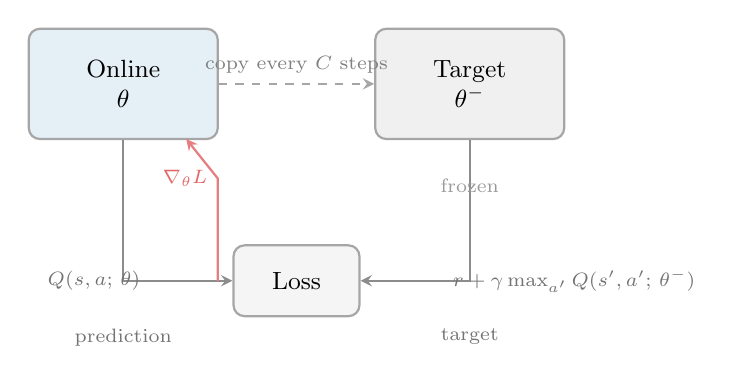
\begin{tikzpicture}[
    net/.style={draw=black!35, thick, rounded corners=4pt,
                minimum width=2.4cm, minimum height=1.4cm,
                font=\small, align=center, inner sep=6pt},
    lossbox/.style={draw=black!35, thick, rounded corners=4pt,
                    minimum width=1.6cm, minimum height=0.9cm,
                    font=\small, fill=black!4},
    arr/.style={->, thick, >=stealth, black!45},
    garr/.style={->, thick, >=stealth, palB!60},
    darr/.style={->, thick, >=stealth, black!35, dashed},
    lbl/.style={font=\scriptsize, text=black!55},
]

% Online network
\node[net, fill=palA!12] (online)
    at (-2.2, 0) {Online\\$\boldsymbol{\theta}$};

% Target network
\node[net, fill=black!6] (target)
    at (2.2, 0) {Target\\$\boldsymbol{\theta}^-$};

% Loss node
\node[lossbox] (loss) at (0, -2.5) {Loss};

% Prediction arrow (online -> loss)
\draw[arr] (online.south) -- (-2.2, -2.5) -- (loss.west)
    node[lbl, pos=0.25, left] {$Q(s, a;\, \boldsymbol{\theta})$};

% Target arrow (target -> loss)
\draw[arr] (target.south) -- (2.2, -2.5) -- (loss.east)
    node[lbl, pos=0.25, right]
    {$r + \gamma \max_{a'} Q(s', a';\, \boldsymbol{\theta}^-)$};

% Gradient arrow (loss -> online)
\draw[garr] (-1.0, -2.5) -- (-1.0, -1.2)
    -- (-1.4, -0.7)
    node[lbl, pos=0.0, left, text=palB!70]
    {$\nabla_{\boldsymbol{\theta}} L$};

% No gradient indicator on target side
\node[font=\scriptsize, text=black!40] at (2.2, -1.3)
    {frozen};

% Copy arrow (online -> target, dashed)
\draw[darr] (online.east) -- (target.west)
    node[lbl, midway, above, text=black!50]
    {copy every $C$ steps};

% Prediction label
\node[lbl, below=1pt] at (-2.2, -2.95)
    {prediction};

% Target label
\node[lbl, below=1pt] at (2.2, -2.95)
    {target};

\end{tikzpicture}
\caption{Target network mechanism. The online network receives
  gradient updates; the target network is frozen and provides stable
  TD targets. Periodically, the online parameters are copied over.}
\label{fig:target-network}
\end{figure}
